\section{Method}
\label{sec:method}
\subsection{From Motion Generation to a Policy}
\label{sec:formulation}
A pretrained motion generator models $p_{\theta}(\mathbf{M}\mid\mathbf{c})$, where $\mathbf{M}$ is a kinematic sequence and $\mathbf{c}$ collects its pretraining conditions. We adapt it into a policy conditioned on instruction $\ell$, egocentric image $I_k$, observed motion history $\mathcal{H}_k$, and bilateral hand state $\mathbf{s}^h_k$:
\begin{equation}
\mathbf{A}_{k+1:k+K}\sim
\pi_{\Theta}(\,\cdot\mid I_k,\ell,\mathcal{H}_k,\mathbf{s}^h_k).
\label{eq:policy}
\end{equation}
Each frame $\mathbf{a}_i=[\mathbf{r}_i,\mathbf{b}_i,\mathbf{h}_i]$ contains root motion, articulated body motion, and two hand-control values. Root and body predictions become kinematic references for SONIC; hand predictions provide synchronized closure commands. The policy executes a prefix before replanning. The generator thus supplies motion structure, while learned conditioning and feedback determine its task-dependent realization.

We use the pretrained Kimodo-G1 denoisers~\cite{kimodo}. Its representation separates global root position and heading from joint positions, velocities, orientations, and foot-contact indicators. With $J$ joints, each frame contains $12J+9$ features. This redundant kinematic representation is converted to tracker references after generation; it is not a vector of motor torques. The supplementary material details its coordinates and components.

\begin{figure*}[t]
\centering
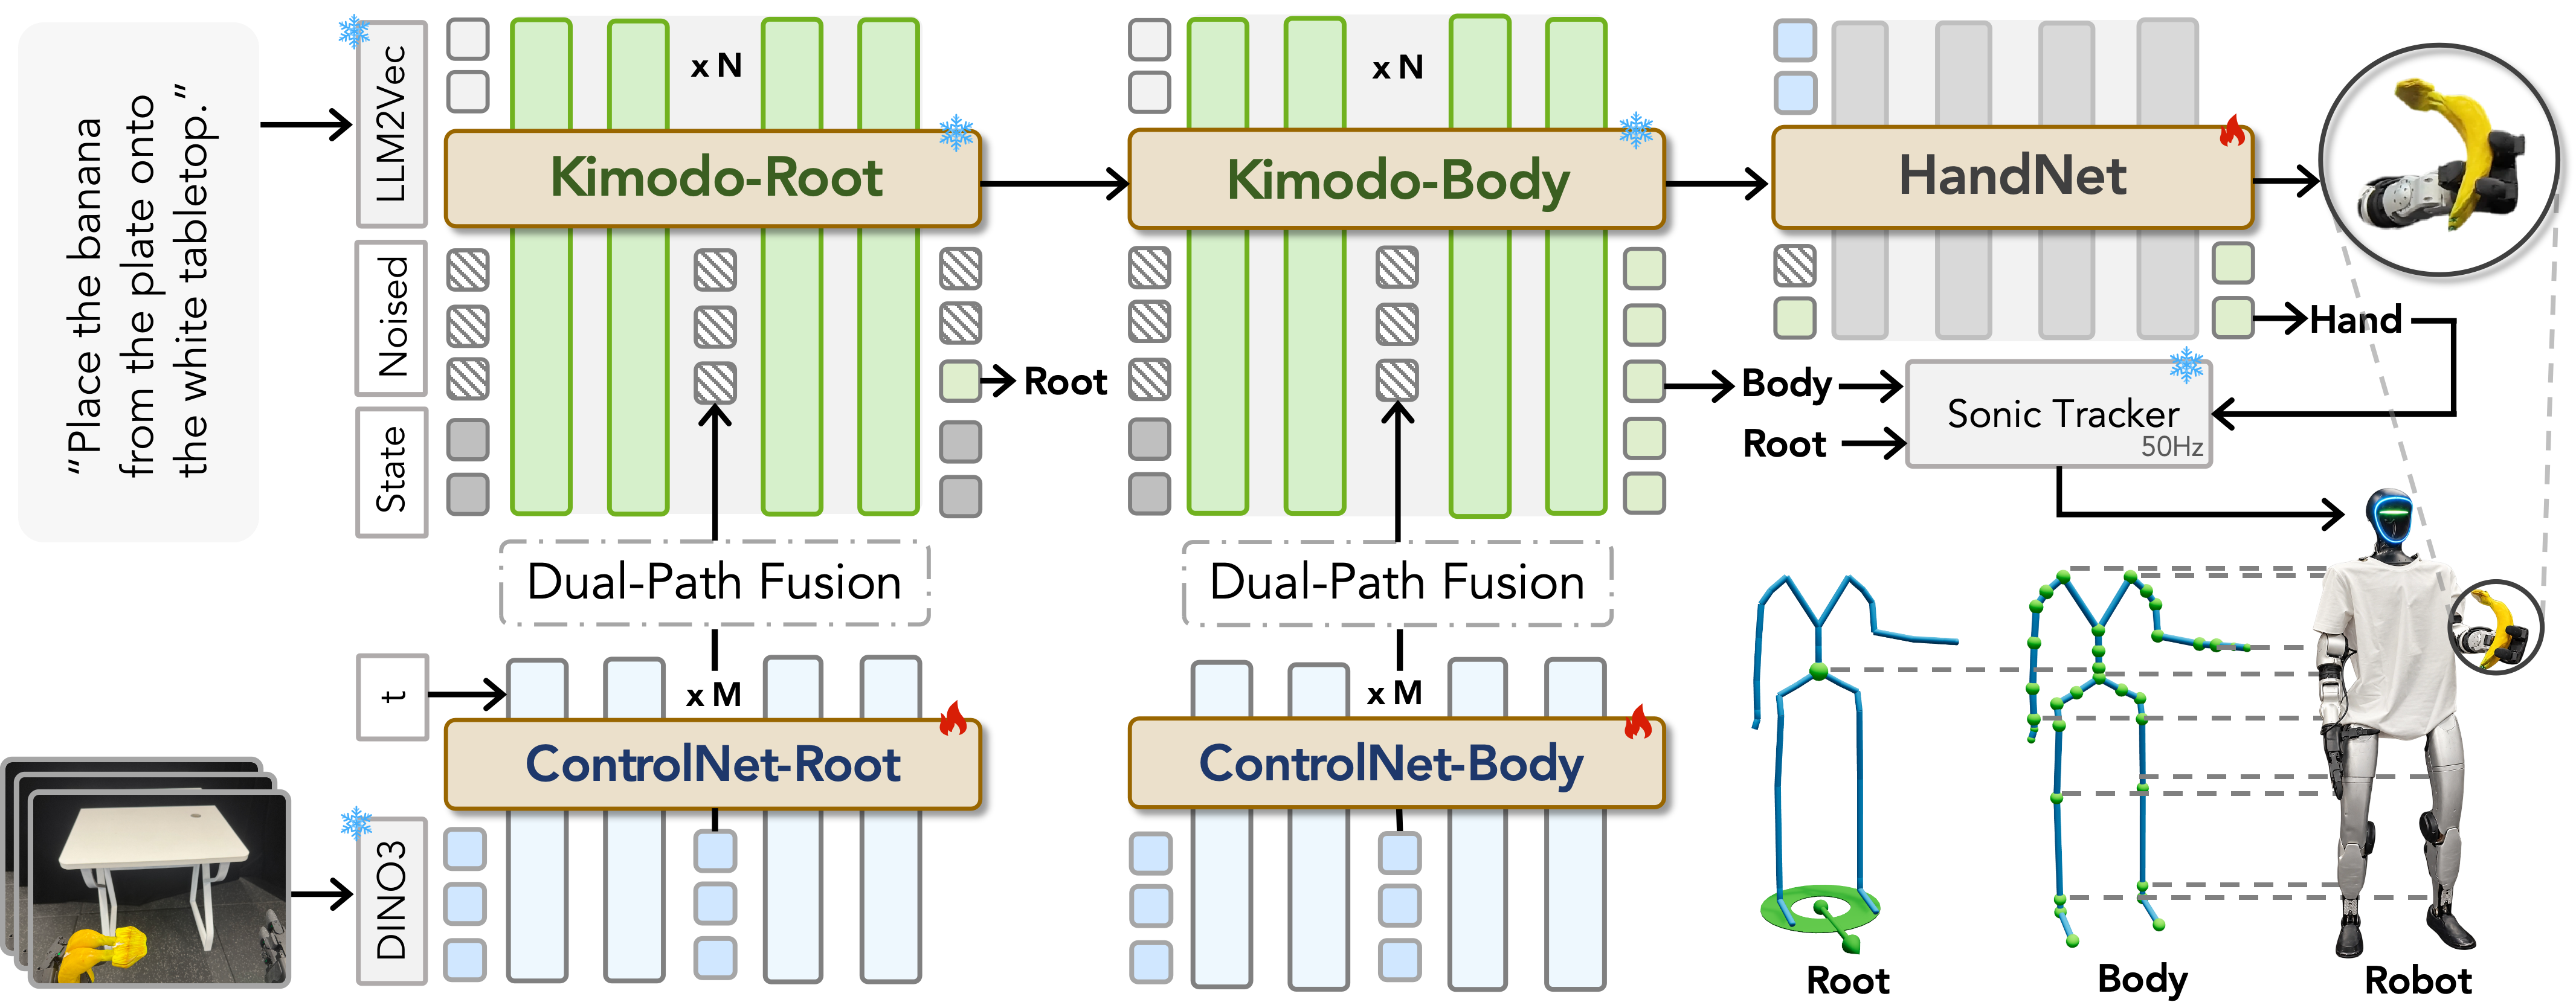
\includegraphics[width=\textwidth]{image/method.png}
\caption{\textbf{Kimodo-Policy.} Frozen Kimodo root and body denoisers receive instruction and motion-history conditioning. Trainable ControlNet branches ground them in DINOv3 image features. Root predictions condition the body, and future body features condition a dedicated HandNet. The motion projector converts generated motion to SONIC tracking references, executed together with hand commands. Snowflakes and flames distinguish frozen and trainable modules.}
\label{fig:architecture}
\end{figure*}

\subsection{Visual Root--Body--Hand Adaptation}
\label{sec:architecture}
\paragraph{Hierarchical generation.}
LLM2Vec~\cite{behnamghader2024llm2veclargelanguagemodels} encodes the instruction and frozen DINOv3~\cite{dinov3} extracts image tokens $\mathbf{V}_k$. We retain the pretrained root and body denoisers, train corresponding ControlNet branches, and add HandNet (Fig.~\ref{fig:architecture}). Let $\mathbf{c}_k$ collect instruction, image, and history conditioning. The stage dependencies are
\begin{align}
\mathbf{z}^r_k &= \mathcal{G}_r(\mathbf{c}_k), \nonumber\\
\mathbf{z}^b_k &= \mathcal{G}_b(\mathbf{c}_k,\sg(\mathbf{z}^r_k)),\\
\widehat{\mathbf{U}}_k &= \mathcal{G}_h(\mathbf{s}^h_k,\sg(\mathbf{V}_k),\sg(\mathbf{z}^b_k)),\nonumber
\label{eq:stages}
\end{align}
where $\mathbf{z}^r_k$ and $\mathbf{z}^b_k$ denote stage predictions and conditioning features, $\sg$ stops gradients, and diffusion noise is omitted. Global root translation and heading are converted to a local representation for body conditioning. HandNet predicts two control values per future frame from current hand state, scene features, and future body features. This organization preserves the pretrained root--body dependency while accommodating the different semantics of hand control.

All root-to-body conditioning is detached, including root ControlNet features. Body losses therefore do not update the root branch. HandNet likewise receives detached body and visual features, so hand supervision updates its own head. These boundaries retain forward coordination while separating optimization across the trainable stages. The frozen backbone alone would not prevent gradients from coupling the trainable control branches; explicit detachment addresses that remaining path.

\paragraph{Dual-path visual fusion.}
At selected denoising layers, a trainable control branch combines two paths from image tokens to future-motion tokens. Cross-attention uses future-motion hidden states as queries, retrieving spatial evidence for each predicted frame. A token-axis MLP maps the image-token sequence to the future horizon, supplying a direct spatial-to-temporal mapping. Their summed features pass through a layer-specific zero-initialized projection and enter the corresponding frozen denoiser as residual hints. Hints affect future tokens only, leaving the constrained history unchanged. Zero initialization preserves the original root/body denoiser output at the start of adaptation, following the ControlNet principle~\cite{zhang2023adding}.

\paragraph{Hand control.}
HandNet is a dedicated diffusion head rather than an extension of the pretrained pose vector. At each denoising step it processes noisy future hand controls, current hand state, future body features, and visual tokens. Binary targets represent opening and closing; continuous targets represent closure changes relative to the latest valid observed hand state. This interface supports different hand embodiments while aligning grasp/release timing with body motion. During policy pretraining, all datasets use a shared two-dimensional binary open/closed representation.

\subsection{History-Constrained Closed-Loop Generation}
\label{sec:history}
Offline motion generation synthesizes a coherent sequence, whereas control must react to tracking error and scene changes after executing only part of a prediction. We formulate each query as constrained completion of a history--future window. Measured motion occupies the prefix; frame- and feature-wise masks mark available values. Before each denoising step, the observed prefix is restored. The model generates only the unconstrained future, with the current image supplying scene information through the visual branches.

The generated root and joint trajectories are converted into tracker-compatible references, and a short prefix is executed alongside the hand controls. The next query uses newly measured motion and an updated image. Consequently, subsequent chunks are anchored to what the robot actually did, rather than only to the previously planned trajectory. Figure~\ref{fig:completion} illustrates the distinction between a full text-conditioned motion and repeated scene-grounded completion. History constraints provide temporal context; they do not guarantee dynamic feasibility, which remains dependent on the tracker and task distribution.

\begin{figure}[t]
\centering
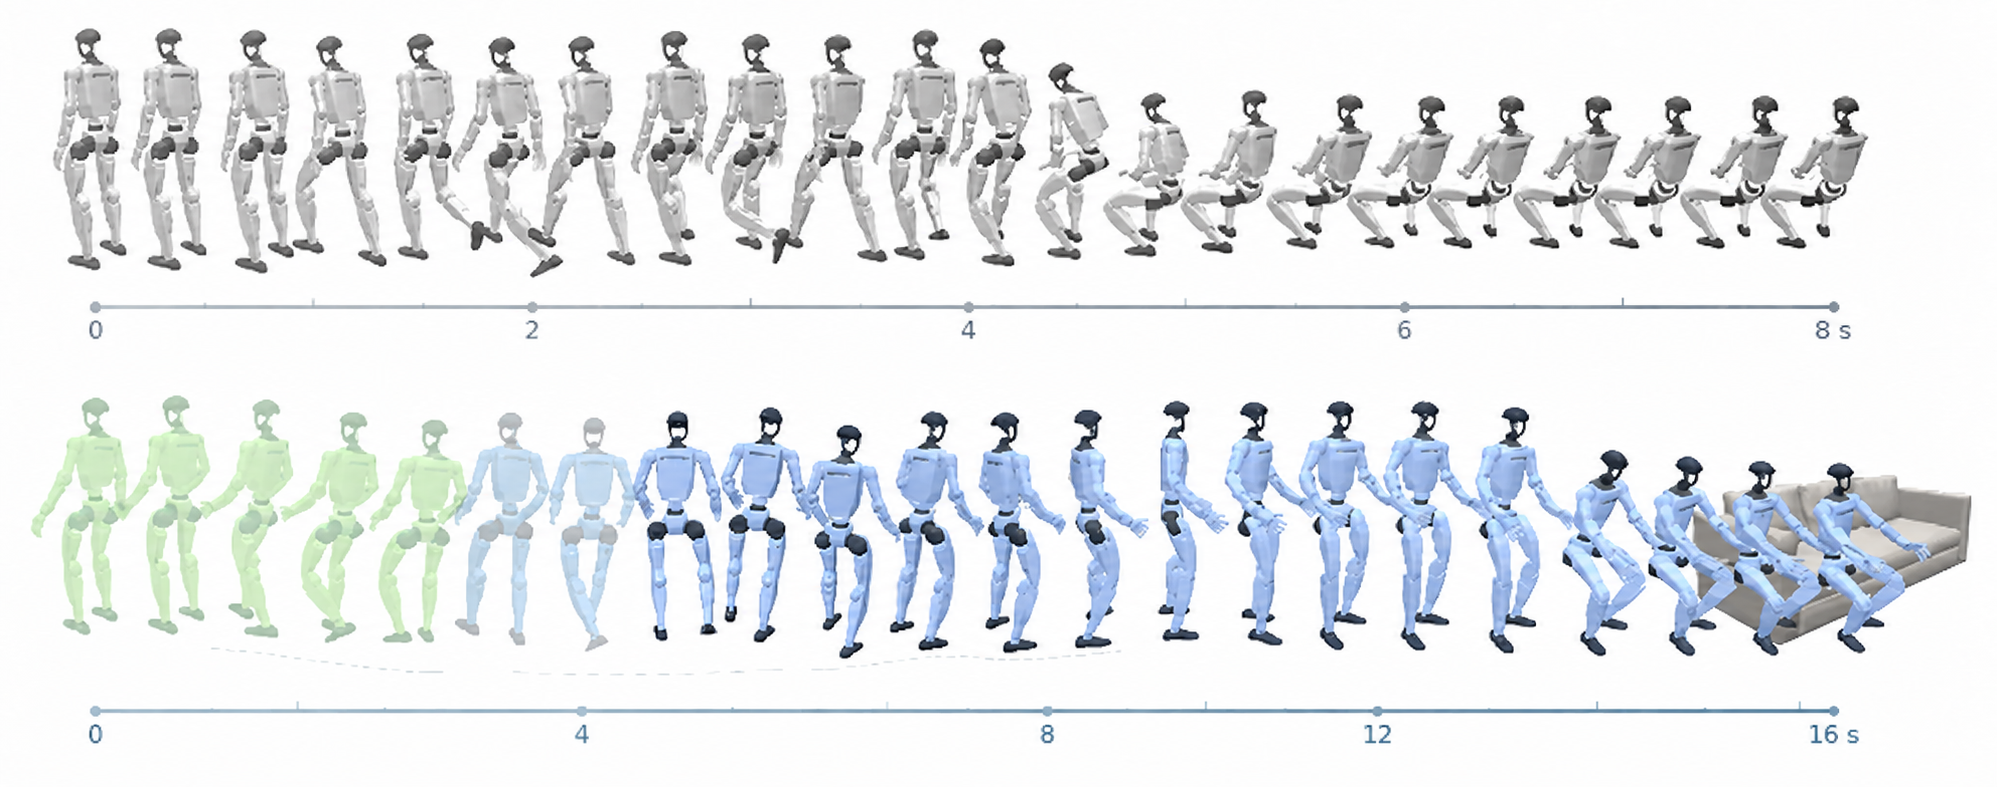
\includegraphics[width=\linewidth]{image/method_222.png}
\caption{\textbf{Motion completion for control.} Top: a text-conditioned sitting sequence from Kimodo. Bottom: scene-grounded generation with observed history (green) and future motion (blue), illustrated for sitting on a sofa.}
\label{fig:completion}
\end{figure}

\subsection{Learning and Execution}
\label{sec:learning}
\paragraph{Objective.}
Training windows pair the current image and instruction with a 100-frame history and 50 future frames sampled at 30\,Hz. We perturb normalized motion features and hand targets with Gaussian noise at a sampled diffusion timestep and supervise clean predictions on valid future frames:
\begin{equation}
\mathcal{L}=4\mathcal{L}_r+\mathcal{L}_b+
\mathcal{L}_h+0.2\mathcal{L}_{\Delta}.
\label{eq:objective}
\end{equation}
Root, body, and hand reconstruction terms are masked mean squared errors. The transition term is the $\ell_1$ error in consecutive hand-control changes, including the boundary from the observed hand state to the first predicted frame. Binary controls are encoded in $[-1,1]$; continuous residuals are converted to closure values before evaluating transitions. Padded motion frames and unavailable hand labels are excluded, with both adjacent labels required for a transition term. Kimodo and DINOv3 remain frozen throughout adaptation.

\paragraph{Two adaptation stages.}
Policy pretraining optimizes visual conditioning and HandNet on 419 hours of heterogeneous humanoid demonstrations. We then fine-tune these trainable modules on the target tasks. We denote direct target-task adaptation as \ours{} and additional policy-pretrained initialization as \ours$^{*}$. Both inherit the pretrained Kimodo motion backbone; the former is therefore not training the whole policy from scratch. This distinction also applies to our real-world comparisons.

\paragraph{Inference.}
We use 10 DDIM denoising steps~\cite{song2022denoisingdiffusionimplicitmodels} on one RTX 4090 and predict 50 motion frames at 30\,Hz. On HumanoidArena and the real robot, 15 frames are executed per update; SIMPLE uses 15 or 50 according to the evaluation setting. SONIC runs at 50\,Hz. Real-time chunking (RTC)~\cite{rtc} is enabled only for physical deployment and disabled in both simulators. Supplementary material gives optimizer settings, data composition, and deployment details.
